\documentclass[a4paper, 11pt]{article}

\usepackage{amsmath}
\usepackage{amssymb}
\usepackage{fancyhdr}
\usepackage{graphicx}
\usepackage{listings}
\usepackage[margin=1in]{geometry}

\lstset{
  basicstyle=\ttfamily,
  mathescape
}

\newcommand{\question}[2] {\vspace{.25in} \hrule\vspace{0.5em}
\noindent{\bf #1: #2} \vspace{0.5em}
\hrule \vspace{.10in}}
\renewcommand{\part}[1] {\vspace{.10in} {\bf (#1)}}

\newcommand{\myname}{Phairat Lin}
\newcommand{\myemail}{phairat.lin@student.mahidol.edu}
\newcommand{\myhwnum}{5}

\setlength{\parindent}{0pt}
\setlength{\parskip}{5pt plus 1pt}
 
\pagestyle{fancyplain}
\lhead{\fancyplain{}{\textbf{HW\myhwnum}}}      % Note the different brackets!
\rhead{\fancyplain{}{\myname\\ \myemail}}
\chead{\fancyplain{}{ICCS200 }}

\begin{document}

\medskip                        % Skip a "medium" amount of space
                                % (latex determines what medium is)
                                % Also try: \bigskip, \littleskip

\thispagestyle{plain}
\begin{center}                  % Center the following lines
{\Large ICCS313: Assignment \myhwnum} \\
\myname \\
\myemail \\
Collaborators: All my friends in 1409
\end{center}

\question{2}{Relational Database Design Theory}
\part{1} \\
Schema:
\begin{verbatim}
    Contracts(c_no, supp_no, proj_no, dept_no, part_no, qty, val)
\end{verbatim}

Alice's findings:
\begin{verbatim}
    c_no -> supp_no proj_no dept_no part_no qty val 
    proj_no part_no -> c_no 
    supp_no dept_no -> part_no 
\end{verbatim}

Bob's findings:
\begin{verbatim}
    c_no -> proj_no supp_no dept_no
    proj_no part_no -> c_no
    supp_no proj_no dept_no -> c_no part_no qty val
\end{verbatim}

No, they are not equivalent. In Alice's findings, You can access part\_no with just supp\_no and dept\_no, but in Bob's findings, you cannot. You need proj\_no in addition to supp\_no and dept\_no to access part\_no. \\
There is no other functional dependency to access part\_no without using proj\_no, which is different from Alice's findings.

\part{2} \\
Let us assume R1 as Table 1 and R2 as table 2. \\
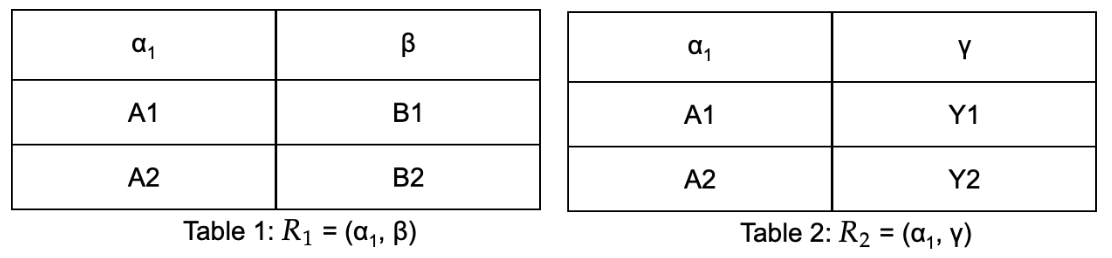
\includegraphics[width=\textwidth]{pic1.png}\\

For the LHS, let us assume R as Table 3. \\
\begin{center}
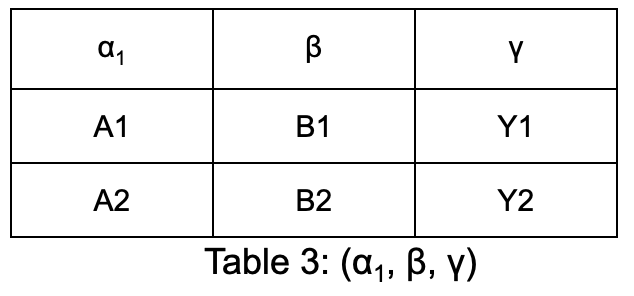
\includegraphics[scale = 0.5]{pic2.png}\\
\end{center}

For the RHS, $R1 \bowtie R2 = \Pi_{A\cup B}(\sigma_{\alpha_1=\alpha_2}(\rho_{\alpha_1\xrightarrow{}\alpha_2}(R1)XR2))\longrightarrow{1}$, as shown in Table 4, Table 5, and Table 6.
\begin{center}
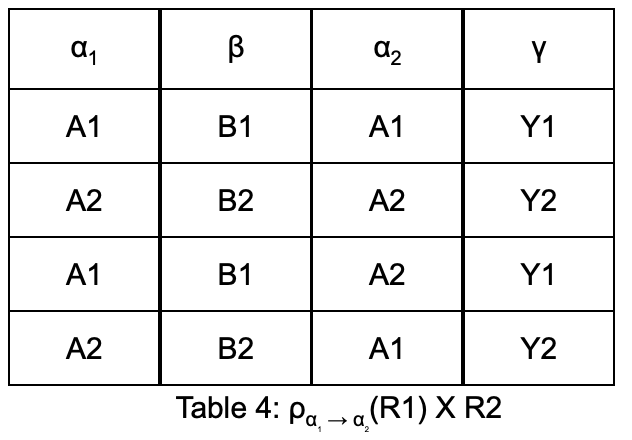
\includegraphics[scale = 0.7]{pic3.png}\\
\end{center}
\begin{center}
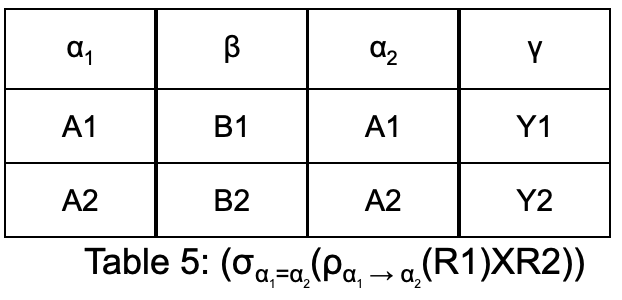
\includegraphics[scale = 0.7]{pic4.png}\\
\end{center}

In Table 6, the union will remove redundancy.
\begin{center}
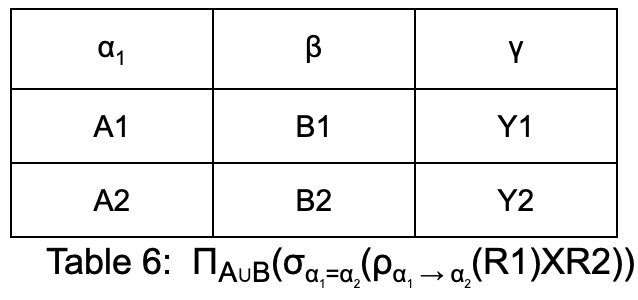
\includegraphics[scale = 0.7]{pic5.png}\\
\end{center}

From this, we can see that Table 6 is equivalent to Table 3 which means $R = R1 \bowtie R2$.

\part{3} \\

\begin{itemize}
    \item No, $R$ is not in BCNF because the determinant CD is not a candidate key.
    \item Decomposing $R$ will give us $R_1$ and $R_2$. $R_1$ will contain BCD and $R_2$ will contain CDA.
    $R_1(BCD)$ 
    \begin{lstlisting}
    Key: BC
    BC $\rightarrow$ D
    \end{lstlisting}

    $R_2(CDA)$
    \begin{lstlisting}
    Key: CD
    CD $\rightarrow$ A
    \end{lstlisting}

    \item No it is not lossless. \\
    If it is lossless, then one of the following will occur: \\
    $$R_1 \cap R_2 \xrightarrow{} R_1$$ 
    $$R_1 \cap R_2 \xrightarrow{} R_2$$ 
    $R_1 \cap R_2 = AC$ \\
    We can check if $AC \xrightarrow{} BCD$ or $AC \xrightarrow{} CDA$ by looking at the closures of all attributes.
    $$AB=\{A, B, C, D\}$$
    $$BC=\{A, B, C, D\}$$
    $$CD=\{A, C, D\}$$
    From the above, we can see clearly that $AC \xrightarrow{} BCD$ or $AC \xrightarrow{} CDA$ is not in the closures, hence it is not lossless.
    
    \item Yes $R$ is in 3NF because even though CD is not a candidate key, A is in the candidate keys which means it is not prime.
\end{itemize}

\question{3}{Storage and Indexing}

\part{1}
\begin{itemize}
    \item Find all tuples of R.\\
    The third approach, scanning through the whole heap file, would most likely require the fewest I/O operations
    \item Find all R tuples such that R.A $\in$ [0, 100)\\
    The first approach, using $B^+$ tree index on R.A., would most likely require the fewest I/O operations due to properties like balanced binary tree.
    \item Find all R tuples such that R.A = 100\\
    The second approach, using hash index on attribute R.A., would most likely require the fewest I/O operations since we obtain the tuples right away, costing $O(1)$ at most.
\end{itemize}

\part{2}
\begin{itemize}
    \item Below is the tree with keys inserted in ascending order.
\begin{center}
    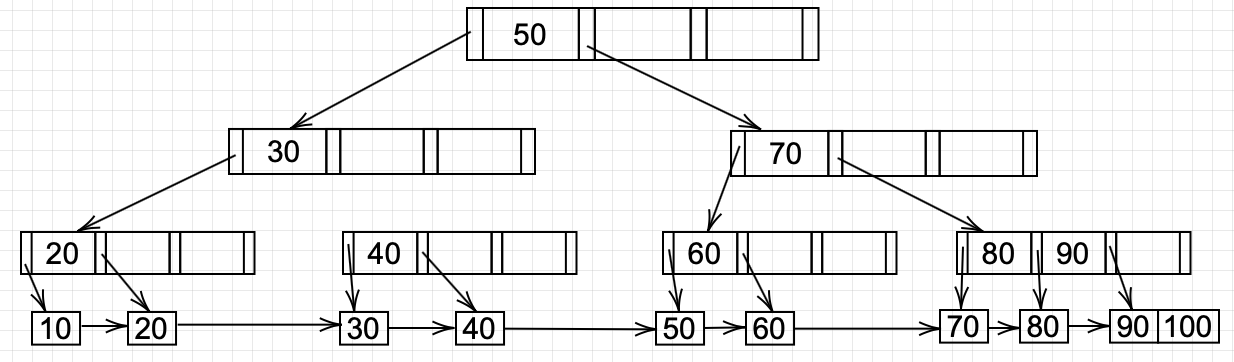
\includegraphics[scale = 0.6]{tree1.png}\\
\end{center}
    \item Yes it is possible by inserting keys in descending order as shown below.
\begin{center}
    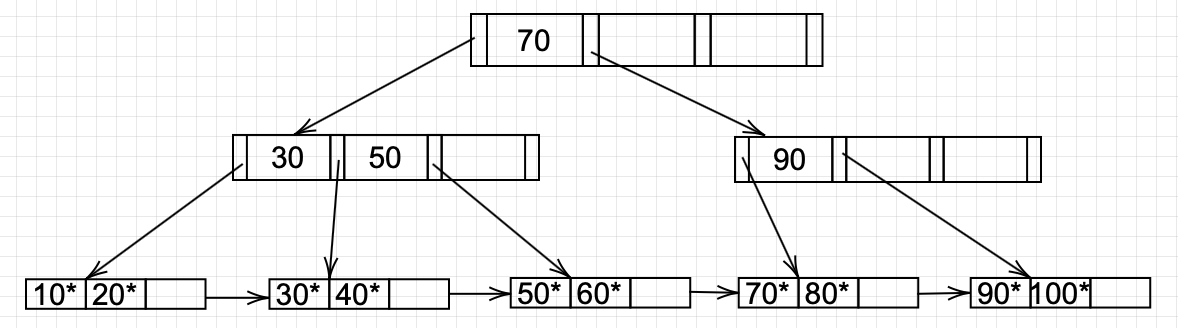
\includegraphics[scale = 0.6]{tree2.png}\\
\end{center}
\end{itemize}

\part{3} \\
\part{a}
\begin{center}
    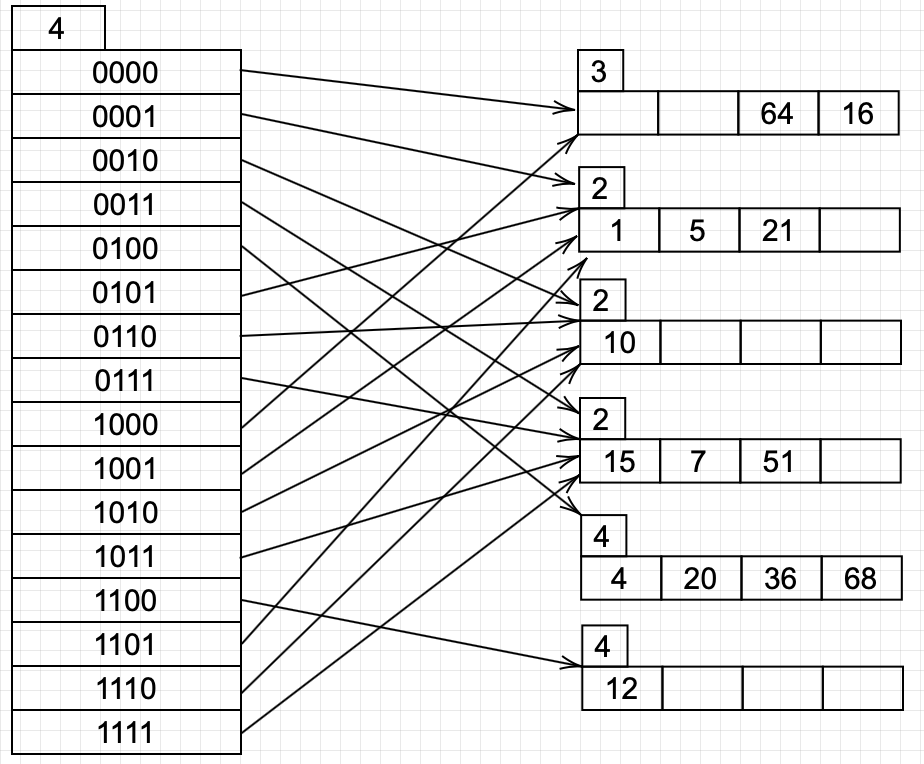
\includegraphics[scale = 0.6]{index.png}\\
\end{center}
\part{b} \\
The minimal set of entries to be deleted from the index that would trigger a merge is \{16, 64\} since it'll result in an empty bucket.







\question{4}{Exam revisited}
\part{1} Set-model will show distinct results, therefore students with the same score will not be shown.

\part{2} 
\begin{verbatim}
SELECT distinct maker 
FROM Computer 
INNER JOIN PC on Computer.model = PC.model	
WHERE speed >= ALL 
(
	SELECT speed 
	FROM PC
) 
\end{verbatim}

\part{3}
The candidate keys are BD and CD because they hold relations to every attribute.

\part{4} \\
$\bullet$
A minimal basis must have single element on the RHS. Since $\mathcal{G}$ has more than one element on the RHS, $\mathcal{G}$ is not a minimal basis of $\mathcal{F}$. \\ 
$\bullet$
Since $A \rightarrow B$ and $A\rightarrow C$ can be combined into $A \rightarrow BC$ and $A \rightarrow BC$ can be split into $A \rightarrow B$ and $A\rightarrow C$, $\mathcal{G}$ is a basis of $\mathcal{F}$ and vice versa. \\
$\bullet$
The minimal basis of $\mathcal{F}$ is $\{A \rightarrow B, A \rightarrow C\}$





\end{document}